\subsection{Retained collection and effective diversity}

All 15,360 scheduled worlds are retained, with 3,072 completed cells per policy and no execution failures. The unchanged auditor verified every SQLite snapshot and recomputed the endpoint summary; a portable artifact recheck agreed. The packaging deviation in Section~IV-D remains part of this result. Across all 120 case--policy groups, none of the recorded endpoint or resource metrics varied over the 128 seeds. Some exogenous timestamps varied, but the repetitions added no endpoint diversity. The substantive challenge set therefore remains 24 authored cases in 12 purposive families, rather than 15,360 independent tasks.

\subsection{Recovery, harms, and the strong comparison}

Every readback policy achieved operational safe recovery in 1,792/3,072 worlds (14/24 cases), compared with 1,024/3,072 (8/24) for response-driven retry. The predeclared equal-family primary difference was $+0.25$. Figure~\ref{fig:recovery-families} shows all 12 family contrasts: three were $+1$, and nine were zero. Differences against the reference, state-only, and one-final-read policies were zero in every family.

The three positive families have specific explanations. In weather-supply and translation-routing cases, response-driven timeout retries created an extra non-idempotent effect; the readback policies dispatched once. In mobile-lab cases, the first response explicitly terminated without an effect; readback policies verified fresh absence and retried, while the response baseline's declared error rule stopped. This third gain concerns that rule, rather than superior deduplication. The equally informed classical reference achieved the same recovery as the package.

\begin{table*}[t]
\caption{Study A: recovery and resources. Each policy has 3,072 planned and completed worlds. Original $D/H$ satisfaction and recovery $R/S$ are distinct targets. Own duplicate and unwanted events can overlap. Means are exact charged counts, not wall latency.}
\label{tab:recovery-outcomes}
\centering\small
\setlength{\tabcolsep}{3.5pt}
\begin{tabular}{lrrrrrrr}
\toprule
Policy & Safe recovery & Original $D/H$ & Recovery $R/S$ & Own duplicate & Own unwanted & Mean reads & Mean dispatches \\
\midrule
Response retry & 1024/3072 & 1280/3072 & 1024/3072 & 1024/3072 & 256/3072 & 0 & $17/12$ \\
Readback state & 1792/3072 & 1792/3072 & 1792/3072 & 256/3072 & 256/3072 & $5/2$ & $5/4$ \\
Separate reference & 1792/3072 & 1792/3072 & 1792/3072 & 256/3072 & 256/3072 & $5/2$ & $5/4$ \\
ConseqaX one final read & 1792/3072 & 1792/3072 & 1792/3072 & 256/3072 & 256/3072 & $5/4$ & $5/4$ \\
ConseqaX polling & 1792/3072 & 1792/3072 & 1792/3072 & 256/3072 & 256/3072 & $5/2$ & $5/4$ \\
\bottomrule
\end{tabular}
\end{table*}

Residual harm is material. In the same 256 archive-rights worlds, one initial provider dispatch created two wrong-payload effects. These are both duplicate and unwanted events, not 512 distinct harmed worlds. Detection did not cancel or repair the effects. Environmental-release cases supply a different failure: an external actor satisfies the original contract, then a delayed own effect breaks the later exact-count target without an own duplicate or unwanted flag. All 256 response worlds with original satisfaction but failed recovery belong to this family. Equal aggregate original/recovery counts for the readback policies conceal a 256-world later-recovery gain and a different 256-world later loss. One target cannot substitute for the other.

All 3,072 reference--polling pairs agreed on final state/linkage reports, endpoint vectors, controller action sequences, and full retained truth. This is observed implementation conformance under the shared policy, not superiority over the strong reference. State-only and polling also had identical actions and physical histories; 1,024 pairs differed in the action-linked report. Provenance expanded reporting here, without a recovery-action benefit.

\subsection{Reporting and the cost of additional polls}

\begin{table*}[t]
\caption{Study A: original-contract final reports. Conditional error is wrong/definite; correct yield is correct/planned. Both positive and negative conclusions count. Comparisons use full-ledger truth, rather than contemporaneous support or the later recovery target.}
\label{tab:recovery-reports}
\centering\small
\setlength{\tabcolsep}{8pt}
\begin{tabular}{lrrrr}
\toprule
Policy & State error & State correct yield & Linked error & Linked correct yield \\
\midrule
Response retry & 1024/1792 & 768/3072 & 768/1792 & 1024/3072 \\
Readback state & 0/2304 & 2304/3072 & 0/1024 & 1024/3072 \\
Separate reference & 0/2304 & 2304/3072 & 0/2048 & 2048/3072 \\
ConseqaX one final read & 0/2304 & 2304/3072 & 0/2048 & 2048/3072 \\
ConseqaX polling & 0/2304 & 2304/3072 & 0/2048 & 2048/3072 \\
\bottomrule
\end{tabular}
\end{table*}

The response policy made 768 false-success and 256 false-negative state reports. The readback policies made no wrong definite state report, but abstained in 768/3,072 worlds. Provenance-aware policies retained 1,024/3,072 linked abstentions; state-only retained 2,048/3,072. Correct negative reports contribute to these yields. Zero wrong original-contract reports did not imply zero harms or guaranteed safe recovery.

Polling and one-final-read agreed on both final claims, dispatches, effect histories, and every non-polling-cost endpoint in all 3,072 pairs. Polling nevertheless consumed 7,680 reads versus 3,840, with mean logical decision time 220 versus 200 ms. These are simulated decision times, not measured production latency. The schedule explains the negative finding: no case with insufficient evidence at $H$ became admissibly known at $H+40$ or $H+80$. Transient limitations either cleared before the first final read or persisted beyond the last opportunity. Thus Study A shows no incremental polling utility under its schedules; it does not test the general benefit of recoverable lag. The separately frozen follow-up below addresses that specific coverage gap.

\begin{figure*}[p]
\centering
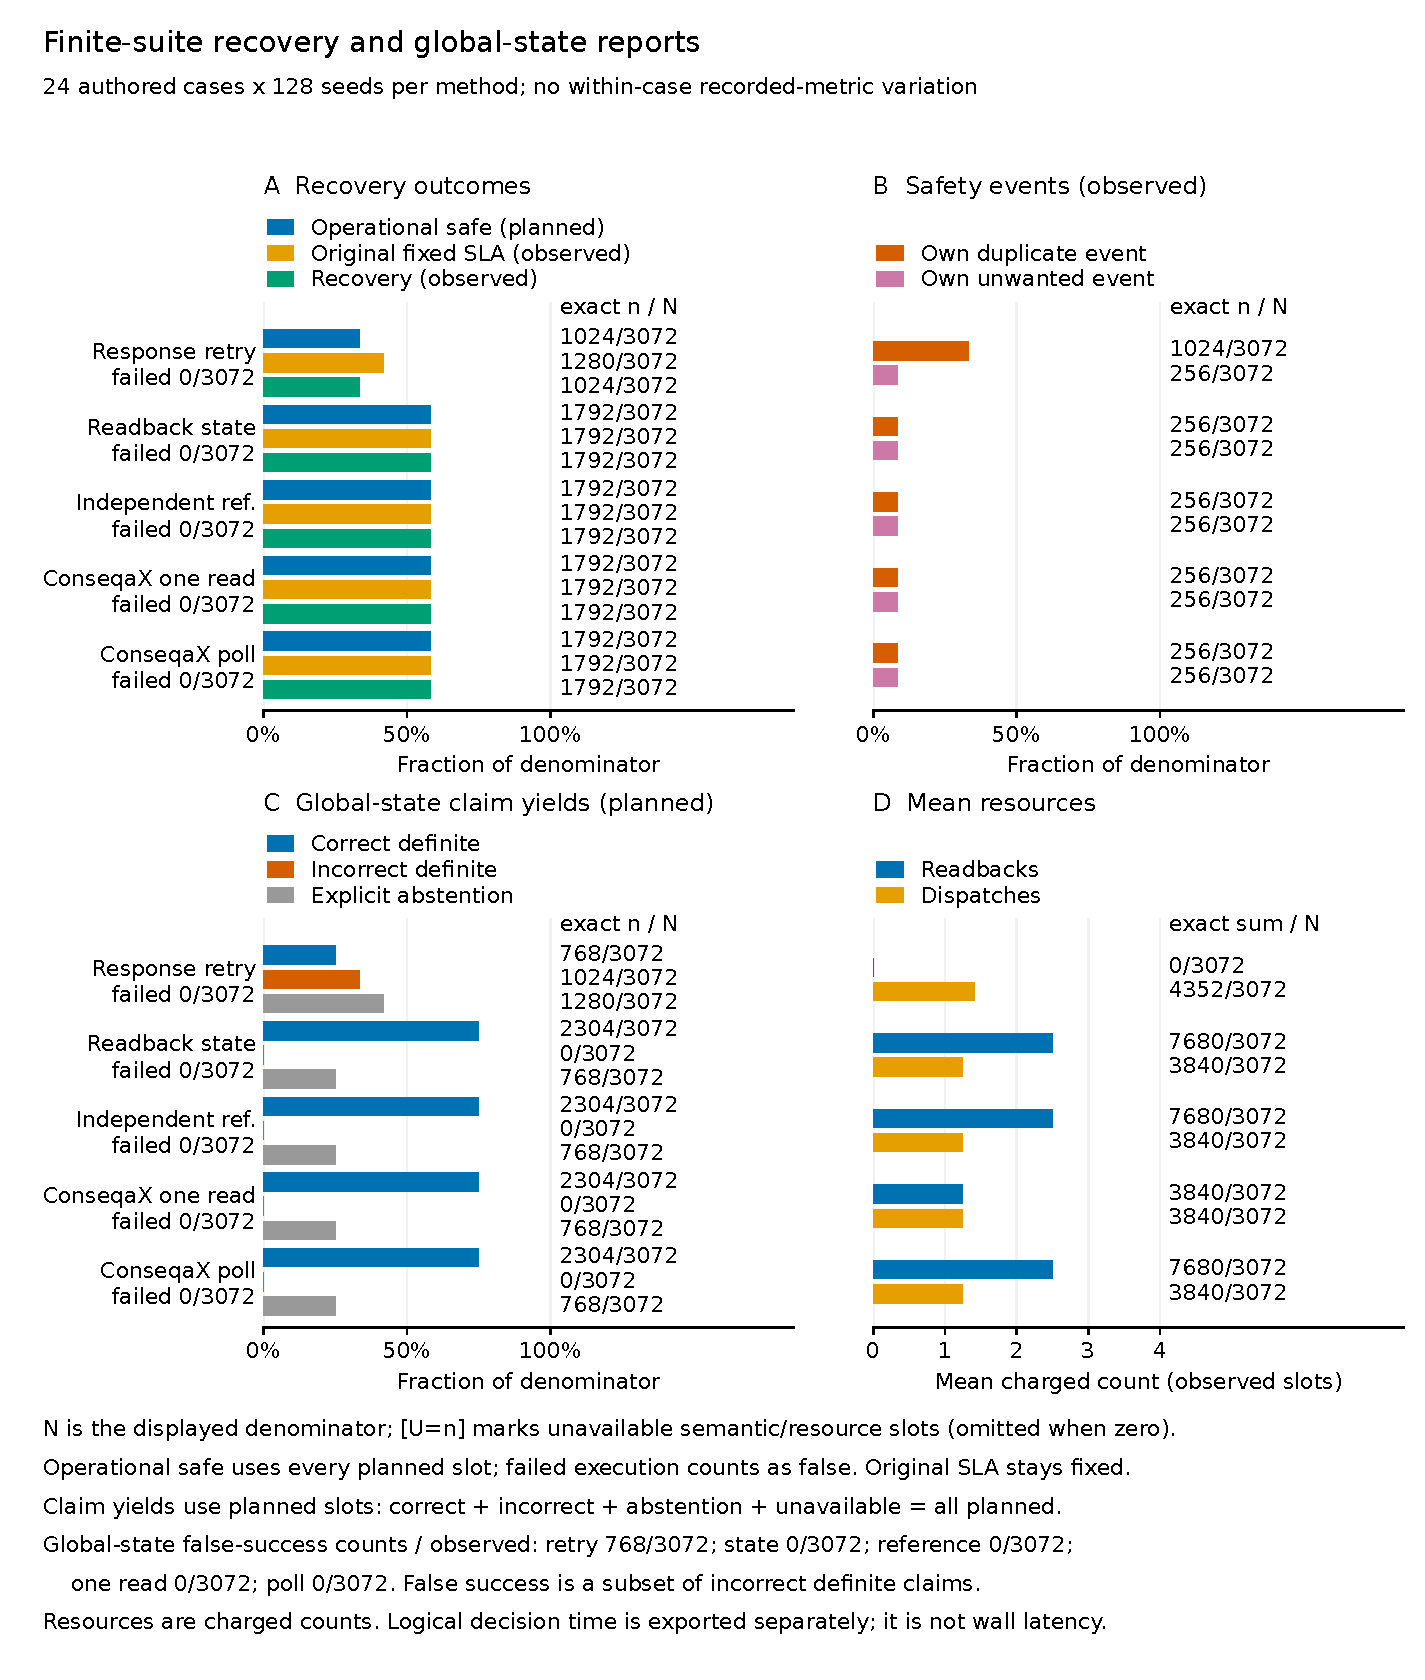
\includegraphics[width=\textwidth,height=0.89\textheight,keepaspectratio]{recovery-method-overview.pdf}
\caption{Study A: all five policies, exact denominators, own harmful events, global-state reporting, and read/dispatch costs. All recorded metrics were constant across seeds within each of the 24 authored cases. Reference independence concerns evidence arithmetic; application transitions and controller authorship are shared. Reporting correctness is distinct from physical recovery and evidence support.}
\label{fig:recovery-overview}
\end{figure*}

\begin{figure*}[t]
\centering
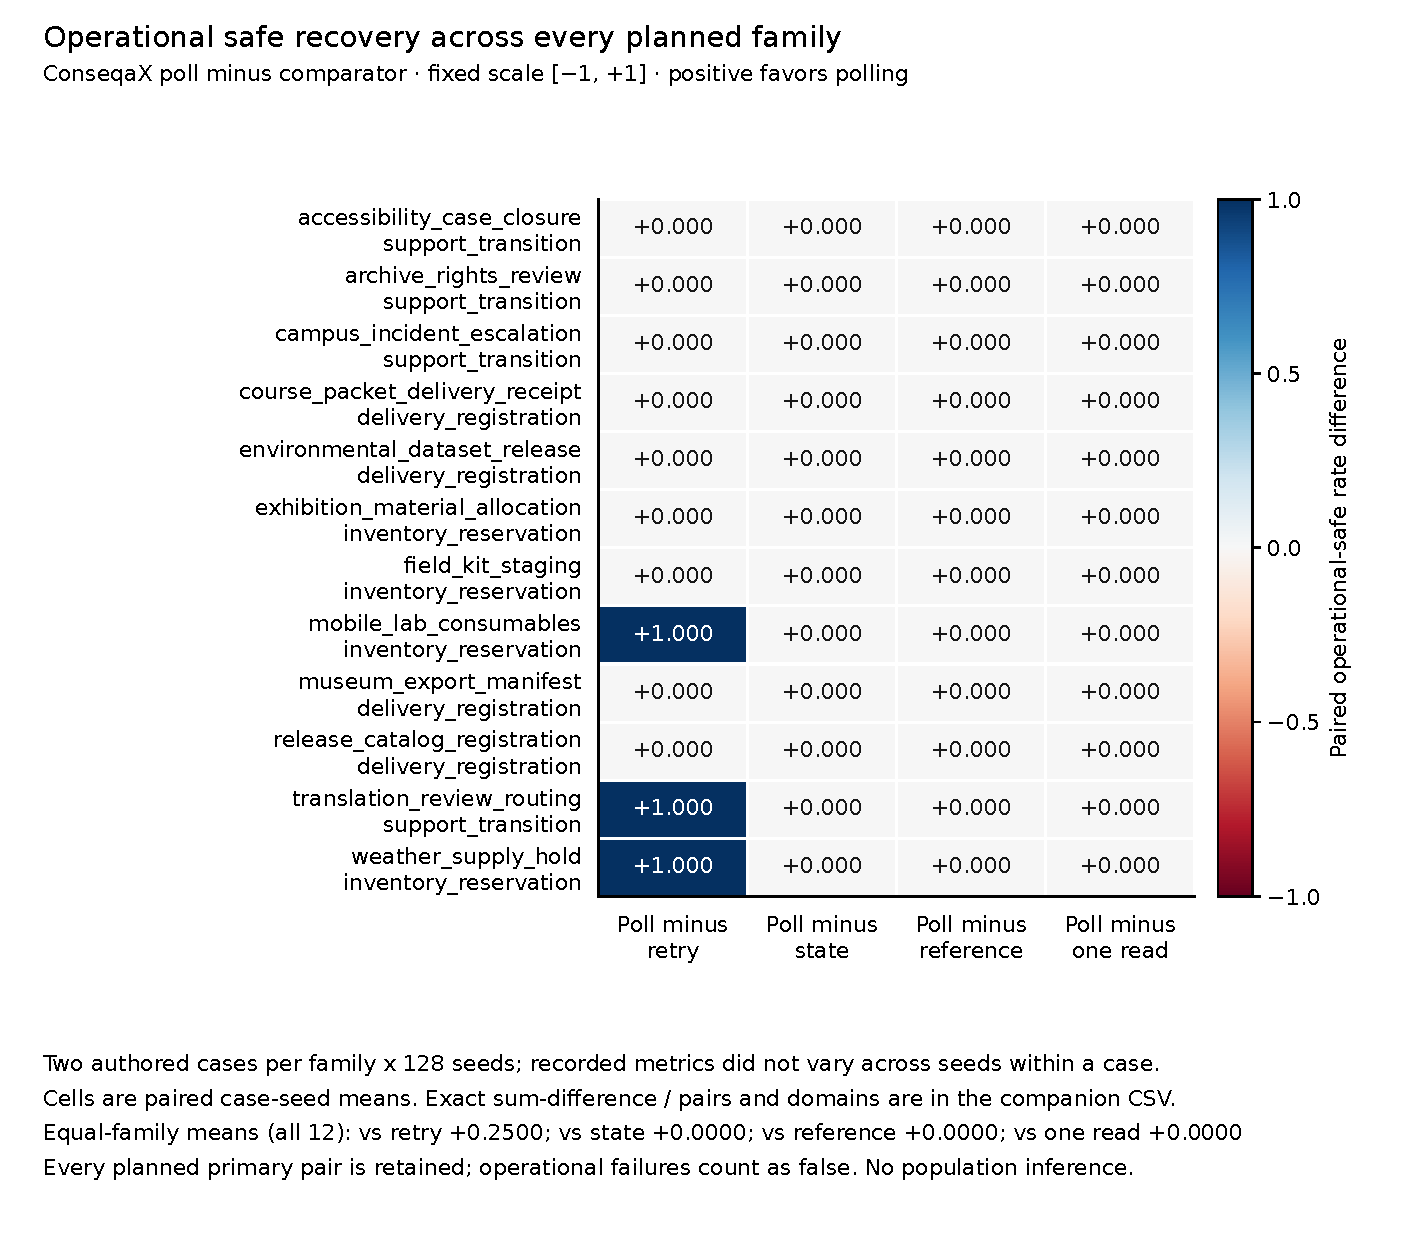
\includegraphics[width=\textwidth,height=0.76\textheight,keepaspectratio]{recovery-family-primary-contrasts.pdf}
\caption{Study A: every planned family's paired operational-safe difference, on a fixed $[-1,1]$ scale. Each family has two related cases and 128 seeds; repetitions added no recorded-metric variation. The equal-family difference is $+0.25$ against response retry and zero against all three readback comparators. These purposive families do not support task-population inference.}
\label{fig:recovery-families}
\end{figure*}

\subsection{Study B: controlled evidence availability}

Study A's coverage gap motivated a separate follow-up after its outcomes were known. We retained the byte-identical world, controllers, and evaluator, then froze a new complete factorial grid before collecting its own data. Source commit \texttt{\seqsplit{d805b3e3560c05ee0a7efd02a80fc18503c6ee05}}, protocol commit \texttt{\seqsplit{b937920469285cdd971783fa6cb33216a7e4da13}}, and protocol SHA-256 \texttt{\seqsplit{e874c6781aa0dbc8ef682ea0a8d37c25d73cc861dada05fd0379116d4a7f6584}} bind that design. This is a disclosed, post hoc motivated sensitivity experiment, rather than a new held-out corpus or replacement for Study A.

The 64 profiles cross readback lag $\{0,40,80,95\}$ ms with independently varied unavailable-until and incomplete-until times $\{0,170,210,250\}$ ms. Each profile repeats in the three domains at seed zero: 192 cases and 960 scheduled policy worlds. Here $D=100$, $H=150$, $R=250$, and $S=330$ ms; reads remain at $50,150,190,230$ ms. Every initial dispatch acknowledges at 2 ms and creates one correct effect at 10 ms. All arms share native idempotency. There are no external writes, removals, or wrong effects. This intentionally uniform physical-success design isolates evidence-window coverage and cost. Profiles are controlled mechanisms, and the three domains repeat them; neither 192 cases nor 960 worlds represent independent task samples.

All 960 worlds completed without failure. The separately implemented auditor verified 1,925 saved artifacts, queried all 960 SQLite snapshots, and agreed with the summary. Unlike Study A, the original collector produced its terminal manifest and receipt normally. All five policies dispatched once, achieved original and recovery satisfaction in 192/192 worlds, and had zero duplicate or unwanted events. Their physical effect histories agreed in every five-arm case. Thus the primary safe-recovery contrast is zero.

\begin{table*}[t]
\caption{Study B: exact finite-grid reports and read costs, 192 planned/completed worlds per policy. Every definite report is hindsight-correct in this uniform-success design. It cannot estimate the response policy's false-success risk. Linked abstention is distinct from state abstention.}
\label{tab:availability-results}
\centering\small
\setlength{\tabcolsep}{4pt}
\begin{tabular}{lrrrrr}
\toprule
Policy & State correct/planned & State unknown & Linked correct/planned & Total reads & Mean decision (ms) \\
\midrule
Response retry & 192/192 & 0/192 & 192/192 & 0 & 2 \\
Readback state & 81/192 & 111/192 & 0/192 & 741 & 224.375 \\
Separate reference & 81/192 & 111/192 & 81/192 & 741 & 224.375 \\
ConseqaX one final read & 3/192 & 189/192 & 3/192 & 192 & 150 \\
ConseqaX polling & 81/192 & 111/192 & 81/192 & 741 & 224.375 \\
\bottomrule
\end{tabular}
\end{table*}

The one-final-read policy resolved one of 64 profiles per domain; polling resolved 27, matching the prospectively specified timing calculation. The paired correct-state-yield increase is $78/192=26/64=0.40625$, shared by the reference and state-only readback. All 192 reference--polling pairs agreed on reports, endpoint vectors, dispatch decisions, and physical records. State-only differed from polling in 81 linked reports while preserving actions and physical outcomes. Polling used 741 reads versus 192 for one-final-read, or 3.859375 versus one per world; mean logical decision time increased by 74.375 ms. These are charged simulated reads and decision times, not production latency.

The full factor grid in Fig.~\ref{fig:availability-grid} shows the boundary: late opportunities help only when availability and completeness recover and the watermark reaches $H$. Lag 95 ms and either window persisting through 250 ms remain unresolved. The ACK-driven response policy reports all 192 successes correctly in hindsight with no read, since all effects are constructed to succeed. Its report arrives before the effect and without horizon-covering evidence; this experiment supplies no estimate of its risk in failing worlds. Together, the studies show conditional polling utility and its cost, with no package superiority over the equally informed reference, no additional recovery-action benefit, and no task-population inference.

\begin{figure*}[p]
\centering
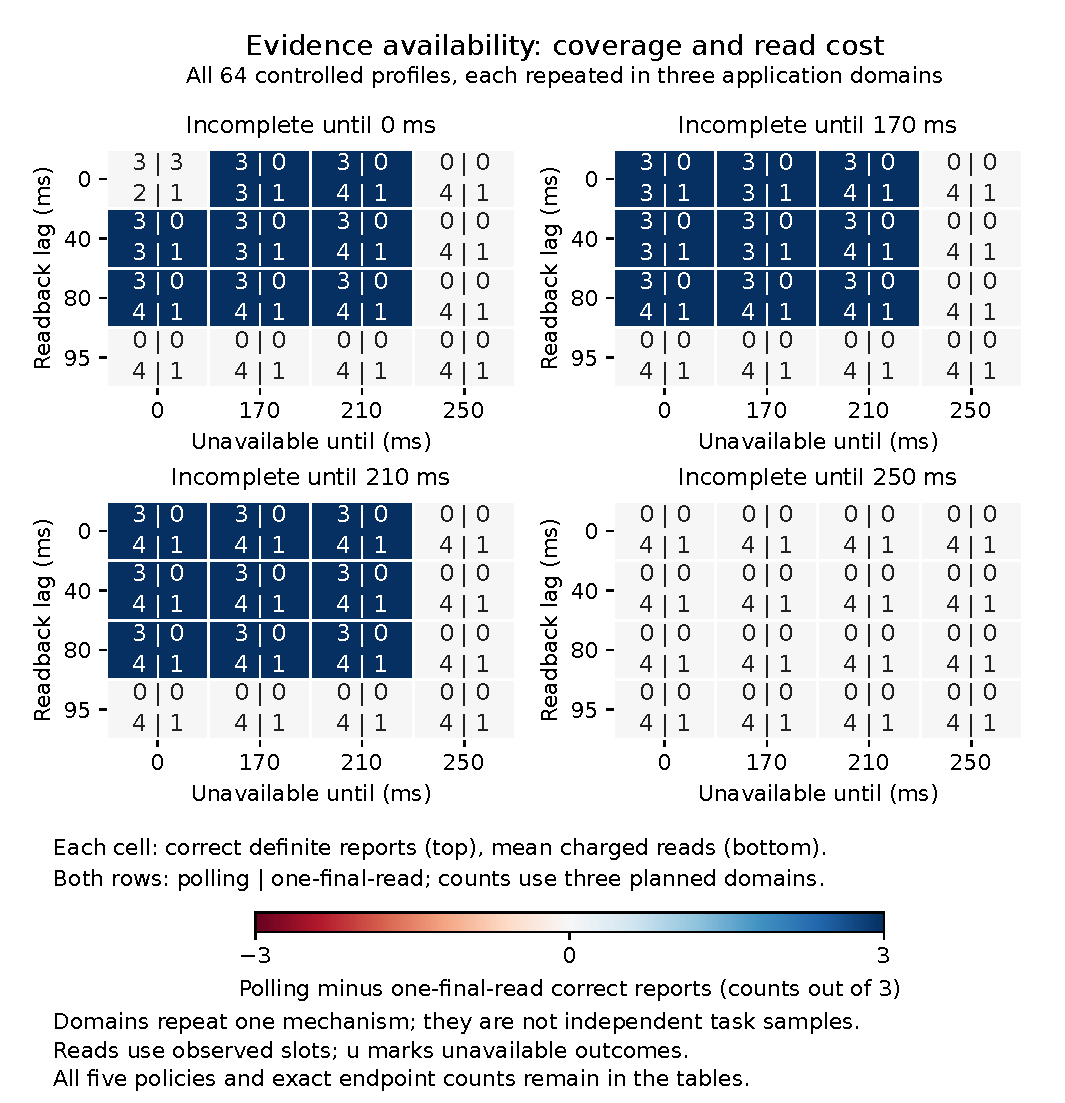
\includegraphics[width=\textwidth,height=0.76\textheight,keepaspectratio]{recovery-availability-grid.pdf}
\caption{Study B: all 64 controlled availability profiles, repeated across three domains. Actual report coverage and read costs are retained for polling and one-final-read. These paired conditions isolate evidence timing; every policy has identical successful physical outcomes, and the classical reference matches polling.}
\label{fig:availability-grid}
\end{figure*}

